\documentclass[a4paper,10pt]{article}
\usepackage[utf8]{inputenc}

\usepackage{url}
\usepackage{graphicx}

%opening
\title{QHY Filter Wheel RS-232 Commands Guide}
\author{Zerjillo \\ (\url{zerjioi@ugr.es})}
\date{}

\begin{document}

\maketitle

\begin{abstract}
This document specify the commands that can be issued to the QHY Filter Wheel\cite{qhyofficial} through the RS-232 interface. Mainly taken from the QHY Official Forums\cite{qhyforum}.
\end{abstract}


\section{The Commands}

The filter wheel admits commands via the RS-232 (serial) interface. It should be set to 9600bps.

\subsection{\texttt{Change Filter} Command}

To change to a specific filter slot (numbered from 0 to 4) a single byte should be sent to the wheel, being:

\begin{itemize}
  \item \texttt{'0'} - for slot 0
  \item \texttt{'1'} - for slot 1
  \item \texttt{'2'} - for slot 2
  \item \texttt{'3'} - for slot 3
  \item \texttt{'4'} - for slot 4
\end{itemize}

Please note that the command refers to the CHARACTERS \texttt{'0'} (\texttt{0x30}) to \texttt{'4'} (\texttt{0x34}), NOT byte values 0 to 4. Once the wheel finishes turning and the correct slot is in place, the wheel will send a \texttt{'-'} (\texttt{0x2D}) character.

The motor only rotates towards one direction to avoid the back space of the gear. For example:

\begin{itemize}
 \item The current position is \texttt{2}; want to goto \texttt{4} $\rightarrow$ the motor will rotate to \texttt{4} (first \texttt{3}, then \texttt{4}).
 
 \item The current position is \texttt{2}; want to goto \texttt{1} $\rightarrow$ the motor will not rotate backwards directly to \texttt{1}, it will rotate to \texttt{3}, \texttt{4}, \texttt{0} and finally to \texttt{1}.
\end{itemize}

In each case, near to position \texttt{0}, the wheel will do a initial calibration. The calibration uses a linear magic sensor. The ADC in the wheel will read the magic intensity and find out the maximum intensity value. This will give a very high precision initial calibration. Please note that it is perfectly normal for the wheel to rotate slower near the calibration position.


\subsection{\texttt{Calibration} Commands}

The following commands allow to tune up the filter wheel in case that the filters do not get perfectly aligned. Probably they are not frequently used unless some displacement of the sensor occurs.

\subsubsection{\texttt{Get Filter Slots Positions} Command}

To get the current positions for each of the filter slots you can send the \texttt{``SEG''} (\texttt{0x53 0x45 0x47}) command. The command returns a 17 byte answer where:

\begin{itemize}
 \item Byte \texttt{0}: \texttt{0x00} (always). Theoretically used to identify among different FW that could be developed by QHY. Currently it identifies the 5 filter one.
 
 \item Bytes \texttt{1-2}: A word (big endian) for the filter slot \texttt{0}.
 \item Bytes \texttt{3-4}: A word (big endian) for the filter slot \texttt{1}.
 \item Bytes \texttt{5-6}: A word (big endian) for the filter slot \texttt{2}.
 \item Bytes \texttt{7-8}: A word (big endian) for the filter slot \texttt{3}.
 \item Bytes \texttt{9-10}: A word (big endian) for the filter slot \texttt{4}.
 \item Bytes \texttt{11-16}: Not useful (in future FW models it may be used for the filter slots \texttt{5}, \texttt{6}, \texttt{7}).
\end{itemize}


\subsubsection{\texttt{Set Filter Slots Positions} Command}

To set the current positions for each of the filter slots you can send the following 20 byte command. This command does not return any information back.

\begin{itemize}
  \item Bytes \texttt{0-2}: \texttt{``SEW''} (\texttt{0x53 0x45 0x57})
  \item Byte \texttt{3}: \texttt{0x00} (always). Theoretically used to identify the 5 filter wheel (may be different when QHY develops other FW models).
  \item Bytes \texttt{4-5}: A word (big endian) for the filter slot \texttt{0}.
  \item Bytes \texttt{6-7}: A word (big endian) for the filter slot \texttt{1}.
  \item Bytes \texttt{8-9}: A word (big endian) for the filter slot \texttt{2}.
  \item Bytes \texttt{10-11}: A word (big endian) for the filter slot \texttt{3}.
  \item Bytes \texttt{12-13}: A word (big endian) for the filter slot \texttt{4}.
  \item Bytes \texttt{14-19}: 3 words (big endian). Not useful until a different FW model is released. Recommended values are \texttt{600} (\texttt{0x02 0x58}), \texttt{700} (\texttt{0x02 0xBC}), \texttt{800} (\texttt{0x03 0x20}). 
\end{itemize}


\subsubsection{\texttt{Return to Factory Settings} Command}

To set the factory settings positions for each filter slot you can send the command \texttt{``SEF''} (\texttt{0x53 0x45 0x46}). This command does not return any information back. The default values for each slot are the following:

\begin{itemize}
  \item Slot \texttt{0}: 85 (\texttt{0x00 0x55})
  \item Slot \texttt{1}: 189 (\texttt{0x00 0xBD})
  \item Slot \texttt{2}: 293 (\texttt{0x01 0x25})
  \item Slot \texttt{3}: 394 (\texttt{0x01 0x8A})
  \item Slot \texttt{4}: 498 (\texttt{0x01 0xF2})
  \item Slot \texttt{5}: 600 (\texttt{0x02 0x58}) (not relevant)
  \item Slot \texttt{6}: 700 (\texttt{0x02 0xBC}) (not relevant)
  \item Slot \texttt{7}: 800 (\texttt{0x03 0x20}) (not relevant)
\end{itemize}

\clearpage 

\section{The \texttt{RS-232} Cable}

In order to control the filter wheel using the RS-232 port you need a proper cable to connect the FW to the computer. You can easily build the cable following the next instructions:

\begin{itemize}
  \item \textbf{Computer side:} You need a DB-9 female connector:
  
  \begin{center}
    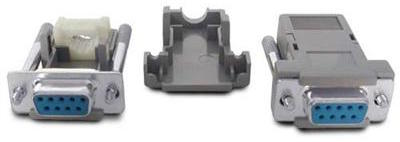
\includegraphics[width=5.5cm]{./DB9_connector.jpg}
    \hfill
    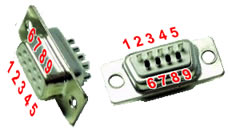
\includegraphics[width=5.5cm]{./DB9_connector02.jpg}
  \end{center}
  
  \item \textbf{Filter Wheel side:} You need a RJ-12 connector:
  
  \begin{center}
    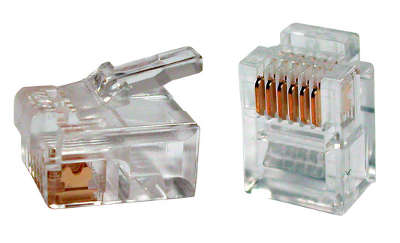
\includegraphics[width=5.5cm]{./rj12.jpg}
    \hfill
    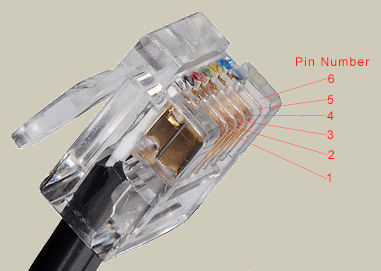
\includegraphics[width=5.5cm]{./rj12_pinout.jpg}
  \end{center}

  \item Solder the following 3 pins on each connector (using some cable, of course):
  
  \begin{table}[h]
  \centering
\begin{tabular}{ | c c c | }
\hline
  \textbf{DB9} & $\longleftrightarrow$ & \textbf{RJ-12} \\ \hline \hline
  2 & $\longleftrightarrow$ & 1  \\ \hline
  3 & $\longleftrightarrow$ & 2  \\ \hline
  5 & $\longleftrightarrow$ & 3  \\ \hline
\end{tabular}
  \end{table}

\end{itemize}


\begin{thebibliography}{9}

\bibitem{qhyofficial}
  QHY Filter Wheel Product Official Web Page \\ \url{http://qhyccd.com/en/left/qhy-colorwheel/}
  
\bibitem{qhyforum}
  QHY Official Forum for the FW \\ \url{http://qhyccd.com/ccdbbs/index.php?topic=1083.0}

\end{thebibliography}

\end{document}
